\documentclass[10pt,a4paper]{article}
\usepackage[margin=0.7in,top=0.6in,bottom=0.65in]{geometry}
\usepackage{amsmath,amssymb,graphicx,booktabs,microtype,hyperref,caption,enumitem,times}
\usepackage{multicol}
\captionsetup{font=footnotesize,skip=2pt}
\setlength{\parskip}{2pt}\setlength{\parindent}{0pt}
\setlist{nosep,leftmargin=1.2em}
\newcommand{\E}{\mathbb E}
\renewcommand{\topfraction}{.9}\renewcommand{\bottomfraction}{.8}\renewcommand{\textfraction}{.07}\renewcommand{\floatpagefraction}{.8}\setcounter{topnumber}{3}\setcounter{totalnumber}{5}
\hypersetup{colorlinks=true,linkcolor=black,citecolor=black,urlcolor=blue}
\title{\vspace{-8mm}\Large\textbf{The Merton Portfolio Problem: How Should Wealth Be Invested Over Time?}\\[-1mm]\large MAC F244: Stochastic Calculus for Finance\vspace{-3mm}}
\author{\normalsize Shrey Rathod (2024ADPS0884G), Harshit Mittal (2024ADPS0849G), Siddh Jain (2024ADPS0837G),\\ Rudraksh Kumar (2024ADPS0820G), Amay Somani (2024ADPS0869G)}
\date{}
\begin{document}\maketitle\vspace{-6mm}
\small
\section{Model and analytic benchmark}
An investor holds a fraction $\pi_t$ of wealth in a risky asset $dS=\mu S\,dt+\sigma S\,dW$ and the rest at the riskless rate $r$, so $dX=[r+\pi(\mu-r)]X\,dt+\pi\sigma X\,dW$, with CRRA utility $U(x)=x^{1-\gamma}/(1-\gamma)$ and horizon $T$. The value function $V(t,x)=\sup_\pi\E[U(X_T)]$ solves the HJB equation \cite{merton69,merton71,oks,pham}
$V_t+\sup_\pi\{[r+\pi(\mu-r)]xV_x+\tfrac12\pi^2\sigma^2x^2V_{xx}\}=0$. The ansatz $V=g(t)x^{1-\gamma}/(1-\gamma)$ gives
\begin{equation}\pi^*=\frac{\mu-r}{\gamma\sigma^2},\qquad V(t,x)=e^{(1-\gamma)\kappa(T-t)}\frac{x^{1-\gamma}}{1-\gamma},\qquad \kappa=r+\frac{(\mu-r)^2}{2\gamma\sigma^2}.\end{equation}
Writing $\rho(\pi)=r+\pi(\mu-r)-\tfrac12\gamma\sigma^2\pi^2$ for the certainty-equivalent (CE) growth rate, $\kappa=\max\rho$ and any other constant fraction loses $\tfrac12\gamma\sigma^2(\pi-\pi^*)^2$ per year.

\textbf{Verification theorem.} Let $\pi$ be admissible (progressively measurable, $\int_0^T\pi_t^2dt<\infty$) and $X=X^\pi$. By It\^o, $dV(t,X_t)=\mathcal L^\pi V\,dt+\pi\sigma XV_x\,dW$, where $\mathcal L^\pi V=V_t+[r+\pi(\mu-r)]XV_x+\tfrac12\pi^2\sigma^2X^2V_{xx}\le0$ by the HJB equation, with equality at $\pi=\pi^*$ (the maximiser, as $V_{xx}<0$). So $V(t,X_t)$ is a local supermartingale for every $\pi$ and a local martingale for $\pi^*$. To pass from local to true: take $\tau_n=\inf\{t:|\ln X_t|\ge n\}\wedge T\uparrow T$; stopped, the stochastic integral is a true martingale, so $\E V(\tau_n,X_{\tau_n})\le V(0,x_0)$. For $0<\gamma<1$, $V\ge0$ and Fatou gives $\E U(X_T)=\E V(T,X_T)\le V(0,x_0)$. For $\gamma>1$, $V\le0$ and Fatou goes the wrong way, so admissibility requires $\{V(\tau,X_\tau)\}_\tau$ to be uniformly integrable (then the limit passes through) \cite[Ch.~3]{pham}. $\pi^*$ is admissible because $V(t,X^*_t)=g(t)(X^*_t)^{1-\gamma}/(1-\gamma)$ is an explicit exponential martingale up to a deterministic factor, so $V(0,x_0)=\E U(X^*_T)$ is attained: $\pi^*$ is optimal and $V$ is the value function.

\textbf{Martingale method (Girsanov).} With $\lambda=(\mu-r)/\sigma$, Girsanov's theorem with density $Z_T=e^{-\lambda W_T-\lambda^2T/2}$ makes $\widetilde W_t=W_t+\lambda t$ a $Q$-Brownian motion, under which $d(e^{-rt}X_t)=e^{-rt}X_t\pi_t\sigma\,d\widetilde W_t$, so discounted wealth is a $Q$-(super)martingale for every strategy. With the state-price density \cite{kls,ks} $\xi_t=e^{-rt}Z_t=e^{-(r+\lambda^2/2)t-\lambda W_t}$ this is the static budget constraint $\E[\xi_TX_T]\le x_0$; maximising $\E[U(X_T)]$ subject to it gives $X_T^*=(y\xi_T)^{-1/\gamma}$ (pointwise concavity bound $U(x)\le U(I(y\xi))+y\xi(x-I(y\xi))$ with $I=(U')^{-1}$, then take expectations), which is exactly the terminal wealth of $\pi^*$. We verified all of this symbolically (HJB residual $=0$, terminal condition, $\nu$ below) and by simulation ($\E[\xi_TX_T]=1.000\pm0.001$ for $\pi\in\{0,.3,.5,1\}$; $\E^Q[W_T]=-3.006$ vs $-\lambda T=-3$; $X^*_T$ equals $(y\xi_T)^{-1/\gamma}$ to $7\!\times\!10^{-16}$). Extensions with closed forms: consumption $c^*=\nu x$, $\nu=[\beta-(1-\gamma)\kappa]/\gamma$; a $[0,1]$ constraint gives the clipped $\pi^*$; and a wealth floor $F$ gives $\pi^*_F=\pi^*(1-Fe^{-r(T-t)}/x)$.

\textbf{$N$ assets.} With $dS_i/S_i=\mu_i\,dt+\sigma_i\,dW_i$, $d\langle W_i,W_j\rangle=\rho_{ij}dt$ (simulated as $W=LZ$, $LL^{\!\top}$ the Cholesky factor of the correlation matrix) and $\Sigma_{ij}=\rho_{ij}\sigma_i\sigma_j$, wealth follows $dX=X[(r+\pi^{\!\top}(\mu-r\mathbf 1))dt+\sum_i\pi_i\sigma_i\,dW_i]$ with $d\langle X\rangle=X^2\pi^{\!\top}\Sigma\pi\,dt$, so the HJB equation is $V_t+\sup_{\pi\in\mathbb R^N}\{(r+\pi^{\!\top}(\mu-r\mathbf 1))xV_x+\tfrac12\pi^{\!\top}\Sigma\pi\,x^2V_{xx}\}=0$. Since $\Sigma\succ0$ and $V_{xx}<0$ the bracket is strictly concave in $\pi$; the first-order condition $(\mu-r\mathbf 1)xV_x+\Sigma\pi\,x^2V_{xx}=0$ gives $\pi^*=-\frac{V_x}{xV_{xx}}\Sigma^{-1}(\mu-r\mathbf 1)=\Sigma^{-1}(\mu-r\mathbf 1)/\gamma$ under the same ansatz. Substituting back gives the one-asset ODE with $(\mu-r)^2/\sigma^2$ replaced by $\theta=(\mu-r\mathbf 1)^{\!\top}\Sigma^{-1}(\mu-r\mathbf 1)$, so $\kappa=r+\theta/(2\gamma)$; $N=1$ recovers (1).

\textbf{Estimation risk} (our central research question). If $\mu$ is estimated from $T_e$ years of data, $\mathrm{se}(\hat\mu)=\sigma/\sqrt{T_e}$ whatever the sampling frequency \cite{merton80} (the sample mean log-return only depends on the endpoints), so $\mathrm{sd}(\hat\pi)=1/(\gamma\sigma\sqrt{T_e})$ and the expected CE loss is $1/(2\gamma T_e)$, and $N/(2\gamma T_e)$ for $N$ assets, independent of correlation. We test this on simulated and on Indian market data. Derivation: $\hat\pi-\pi^*$ is Gaussian with variance $1/(\gamma\sigma)^2T_e^{-1}$, so $\E[\tfrac12\gamma\sigma^2(\hat\pi-\pi^*)^2]=\tfrac{\gamma\sigma^2}{2}\cdot\tfrac1{\gamma^2\sigma^2T_e}$.

\section{Numerical methodology}
\textbf{Monte Carlo.} Parameters $\mu=12\%$, $\sigma=20\%$, $r=6\%$, $\gamma=3$, $T=10$ ($\pi^*=0.5$). Wealth is simulated with Euler--Maruyama (EM) and Milstein \cite{kp,glass}, and compared with the exact solution $X_T=x_0\exp\{(r+\pi(\mu-r)-\tfrac12\pi^2\sigma^2)T+\pi\sigma W_T\}$ on the same Brownian path (strong error: $T{=}1$, $2\!\times\!10^5$ paths, $N=2,\dots,256$ steps, log--log regression on $\Delta t$). Weak error: $|\E U(X^N_T)-\E U(X_T)|$ with $2\times10^6$ paths and common random numbers (the difference $U(X^N_T)-U(X_T)$ on one Brownian path has a tiny variance, so an $O(\Delta t)$ bias is visible far below the plain MC error), plus a noise-free check: one-step moments of both schemes are polynomial in $\Delta t$, so $\E X^N_T$, $\E (X^N_T)^2$ follow exactly by recursion ($N\le256$; MC at $N{=}4$ agrees, $z{=}0.19$). $\E U(X_T)$ uses $10^{6}$ exact terminal draws per strategy; the MC error is regressed on $M\in[10^3,10^6]$.

\textbf{Finite differences.} Substituting $y=\ln x$, we solve the HJB equation in $(t,y)$ with an implicit time step and a hybrid central/upwind discretisation of the drift (central when the diffusion dominates, $a\ge|b|h$, upwind otherwise, to keep the matrix an M-matrix), with the optimal control updated by Howard policy iteration (about 3 iterations per time step). Constraints enter as bounds on the control. \textbf{Dynamic programming.} A discrete Bellman recursion \cite{samuelson} on $N$ rebalancing dates, optimising $\pi$ at each node by parabolic refinement on a grid, with Gauss--Hermite quadrature (24 nodes) for the lognormal step and cubic-spline interpolation in $\ln x$. Exact formulas from Part~1 are used only to measure error.

\textbf{Data.} NSE's official daily Nifty~50 Total Returns Index (dividends reinvested) \cite{nifty}, 17-Sep-2007 to 13-Nov-2026 (4746 returns, 19.2\,y), downloaded from niftyindices.com and checked against an independent price series (all 4554 common days present, daily return correlation $0.99993$) and NSE-official weekly closes \cite{tapetide} (correlation $\ge0.999$). The constant-yield proxy we first used (price index $+1.3\%$) overstated growth by $0.14$ points a year (actual dividend yield $1.17\%$). Risk-free rate: RBI 91-day T-bill auction cut-off yields \cite{rbi}, weekly (1753 auctions, 1993--2026; $2.9$--$12.0\%$ over our sample), each trading day using the latest auction already held (no look-ahead); mean $6.4\%$ over 2007--2026 and $5.5\%$ over the evaluation period (Sep-2017--Nov-2026). We also rerun with constant $r\in\{5,6,6.5,7,8\}\%$ on the same period. Estimation: $\hat\mu=\bar m+\tfrac12\hat\sigma^2$ with log-return mean $\bar m$; $\mathrm{se}$ as above; Ljung--Box and Jarque--Bera tests. Rolling backtest with 3/5/7/10-year windows, monthly rebalancing, 111 dates Sep-2017--Nov-2026, rules: \emph{raw} $\hat\pi$; \emph{capped} to $[0,1]$; \emph{shrunk} (Bayesian: data-weighted $\hat\mu$ and a prior equity premium of $5\%$ with prior s.d.\ $4\%$); \emph{shrunk+capped}.
\textbf{Multi-asset.} NSE's official daily Total Returns Indices for Nifty~50, Bank, IT, FMCG, Pharma over the same 19.2 years (4746 returns); $r=6.4\%$ (mean RBI T-bill yield) for full-sample weights; added one at a time; sample vs Ledoit--Wolf covariance \cite{lw}; unconstrained, long-only and long-only-no-leverage (SLSQP) optimisers; CAPM-implied drifts $\mu_i-r=\beta_i\cdot5\%$ as an alternative; synthetic two-asset correlation experiment; a 5-asset out-of-sample study with known truth; and a rolling real-data backtest with the same period, rebalancing, time-varying $r$ and metrics as Part~1.

\section{Results}
\begin{figure}[!htb]\centering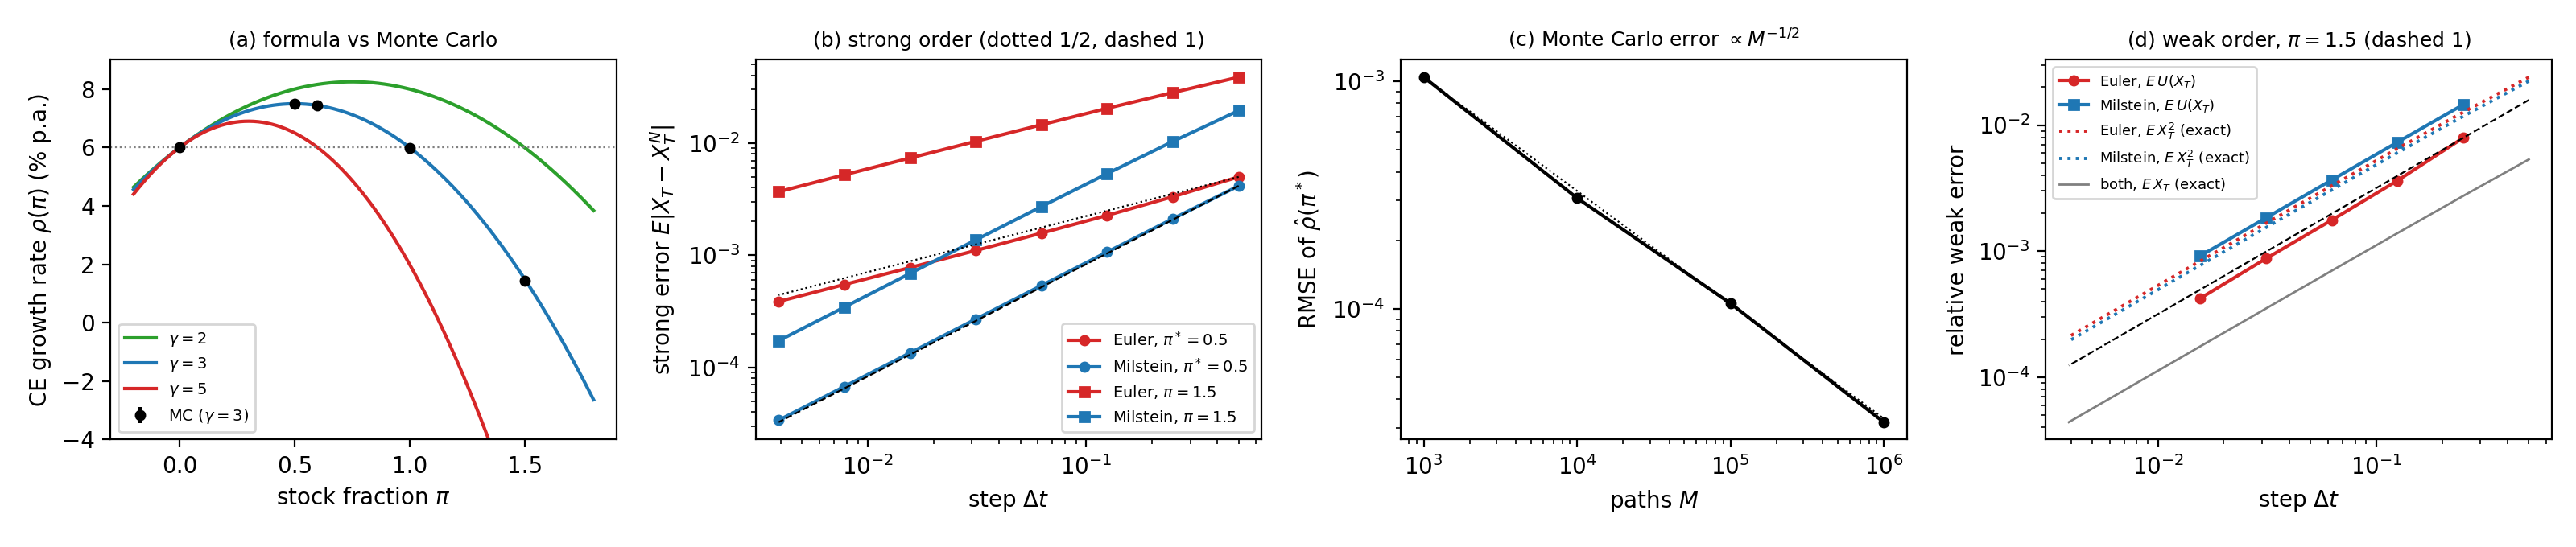
\includegraphics[width=\linewidth]{../figures/fig_mc.png}\caption{Monte Carlo (Part 2): (a) CE growth $\rho(\pi)$, formula vs simulation; (b) strong error vs $\Delta t$ (EM slope $\tfrac12$, Milstein 1); (c) MC rmse vs $M$; (d) weak error vs $\Delta t$ (slope 1; dotted, grey: exact moments).}\end{figure}
\textbf{Verification of the theory by simulation.} Simulated $\E U(X_T)$ agrees with the closed form for all five strategies (largest $|z|=2.2$ for $1.5\times$ leverage whose terminal utility has a very heavy tail; others $|z|<1.5$). Merton's $\pi^*$ has the highest CE growth ($7.50\%$ vs $7.44\%$ for 60/40, $6.0\%$ for all-in, $1.4\%$ at $1.5\times$). Strong order is $0.52$ for EM and $0.99$ for Milstein ($0.49$/$0.98$ at $1.5\times$), error constants shrinking by a factor 15--20 for Milstein at $\pi=1.5$. Weak order is $1.01$/$1.00$ (EM/Milstein) at $\pi^*$ and $1.05$/$1.00$ at $1.5\times$, and $0.98$--$0.99$ from the exact moment recursion: Milstein improves pathwise accuracy but leaves the accuracy of expectations unchanged, so for expected utility the cheaper EM scheme is just as good. MC rmse slope in $M$ is $-0.50$. \textbf{Estimation loss} (not plotted) from $4\!\times\!10^5$ simulated histories matches $1/(2\gamma T_e)$ to within about 1\% (e.g.\ $0.0561$ vs $0.0556$ at $T_e=3$, $0.0167$ vs $0.0167$ at $T_e=10$); for $T_e=3$, $\hat\pi>1$ in 30\% and $\hat\pi<0$ in 30\% of histories; clipping to $[0,1]$ cuts the loss from $0.056$ to $0.011$. \textbf{Parameter sweep} (Fig.~2): $\pi^*$ falls as $1/\gamma$ and $1/\sigma^2$ and is linear in $\mu-r$; leverage ($\pi^*>1$) needs low $\gamma$ or low $\sigma$. Horizon does not matter: simulated $\rho(\pi^*)$ is $7.50\%$ to $\pm0.01\%$ for $T\in\{1,5,20\}$ (the Merton rule is myopic).
\begin{figure}[!htb]\centering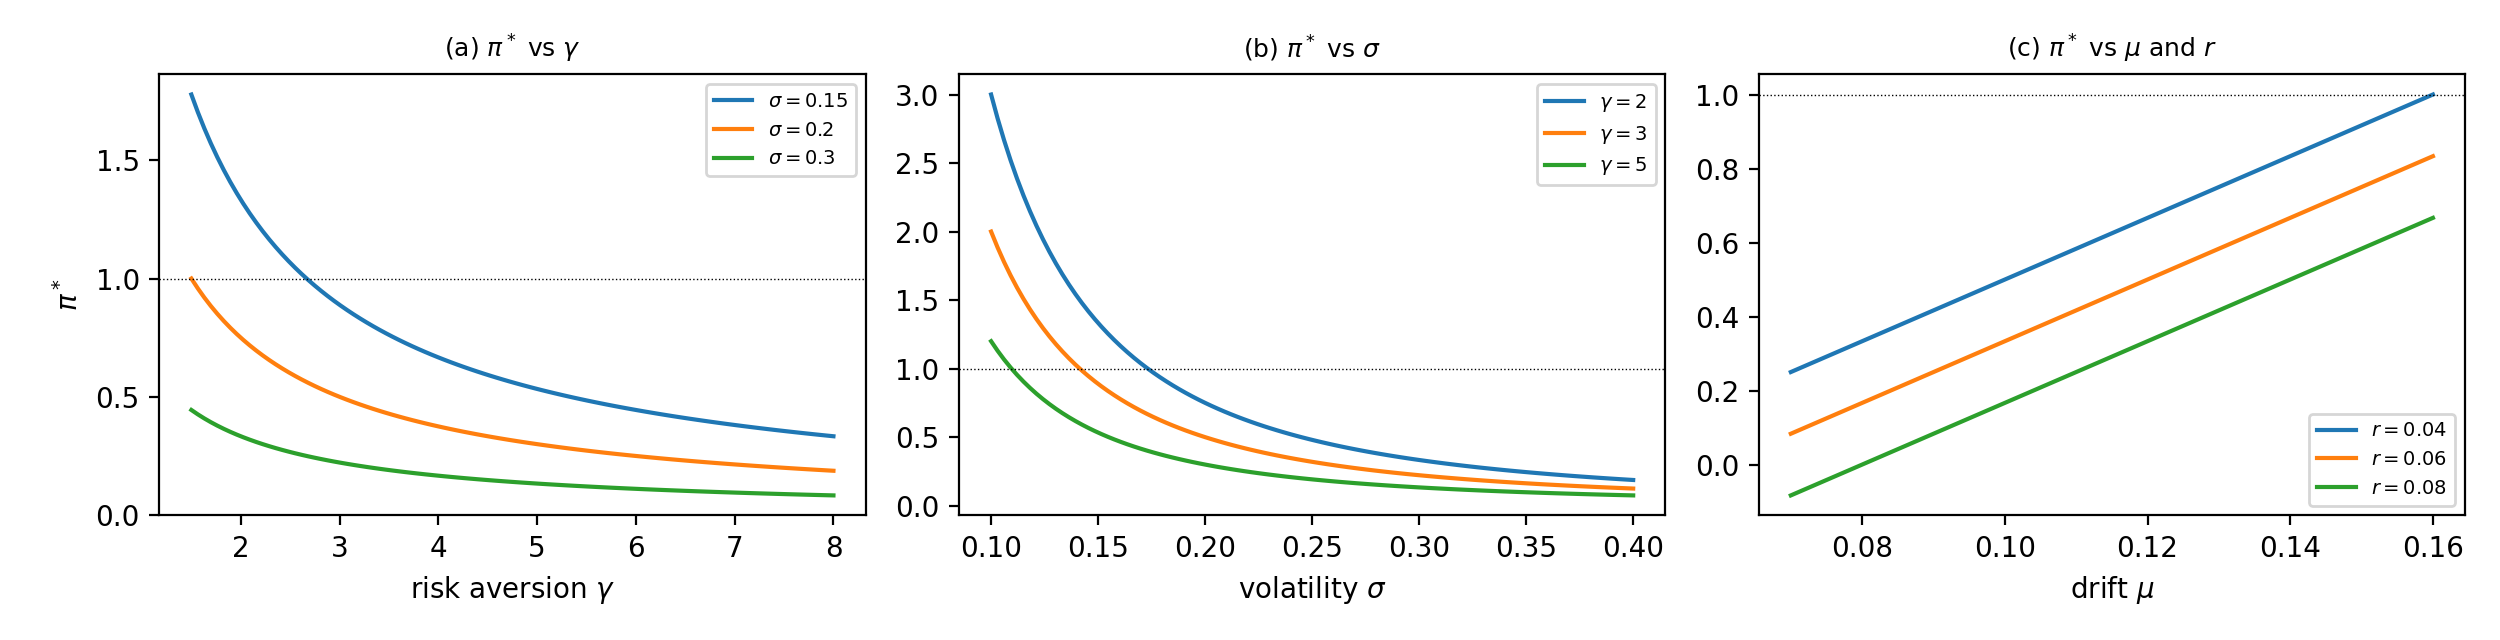
\includegraphics[width=0.8\linewidth]{../figures/fig_sweep.png}\caption{Parameter sweep (closed forms; full grid in \texttt{part2\_param\_sweep.csv}): $\pi^*$ against $\gamma$, $\sigma$, and $\mu$ for three values of $r$; $\pi^*>1$ (above the dotted line) means leverage.}\end{figure}

\begin{table}[!htb]\centering\footnotesize\caption{Numerical HJB/DP vs.\ analytic benchmark. FD: $h=\Delta y$, $N_t=320$; time rows use $h=0.025$, errors against a fine-time reference.}
\begin{tabular}{lll}\toprule
 & FD ($\gamma{=}3$): rel.\ err.\ $V_0$ / err.\ $\pi_0$ & DP ($\gamma{=}5$): rel.\ err.\ $V_0$ / err.\ $\pi_0$\\\midrule
coarse & $h{=}0.2$: $3.1\!\times\!10^{-2}$ / $4.4\!\times\!10^{-3}$ & $N{=}1$: $3.4\!\times\!10^{-4}$ / $1.5\!\times\!10^{-3}$\\
mid & $h{=}0.05$: $2.3\!\times\!10^{-4}$ / $2.8\!\times\!10^{-4}$ & $N{=}4$: $9\!\times\!10^{-5}$ / $3.9\!\times\!10^{-4}$\\
fine & $h{=}0.00625$: $3\!\times\!10^{-5}$ / $<10^{-5}$ & $N{=}52$: $<10^{-5}$ / $2\!\times\!10^{-5}$\\
order & $\pi$: 2.00 (space), $V$: 1.03 (time) & $V$: 1.01, $\pi$: 0.98\\\bottomrule\end{tabular}\end{table}
\begin{table}[!htb]\centering\footnotesize\caption{Accuracy vs run time on the same problem ($\gamma{=}5$, $\pi^*{=}0.3$, $T{=}1$), errors against the closed form (single laptop core).}
\begin{tabular}{llrll}\toprule
method & setting & time (s) & rel.\ err.\ $V_0$ & err.\ $\pi_0$\\\midrule
FD & $h{=}0.025$, $N_t{=}80$ & 0.06 & $7.6\!\times\!10^{-6}$ & $2.0\!\times\!10^{-4}$\\
FD & $h{=}0.0125$, $N_t{=}320$ & 0.16 & $2.0\!\times\!10^{-6}$ & $5.0\!\times\!10^{-5}$\\
FD & $h{=}0.00625$, $N_t{=}1280$ & 0.62 & $4.9\!\times\!10^{-7}$ & $1.2\!\times\!10^{-5}$\\
DP & $N{=}12$ & 0.48 & $2.8\!\times\!10^{-5}$ & $1.3\!\times\!10^{-4}$\\
DP & $N{=}52$ & 1.85 & $3.2\!\times\!10^{-7}$ & $1.6\!\times\!10^{-5}$\\
DP & $N{=}252$ & 8.24 & $1.3\!\times\!10^{-5}$ & $7.6\!\times\!10^{-5}$\\\bottomrule\end{tabular}\end{table}
\textbf{HJB/DP.} The FD control converges at second order in space and the value function at first order in time (backward Euler), matching theory; $V$ error in space saturates at $\sim\!3\!\times\!10^{-5}$ (time-error floor). DP with $N$ rebalancings has error $O(1/N)$ in both $V$ and $\pi$ because the discretely rebalanced optimum differs from the continuous one by $O(\Delta t)$. At $\gamma{=}3$ the DP optimum equals $\pi^*$ exactly ($0.5000$) at every $N$: the rebalancing correction vanishes by coincidence at this parameter set (we checked with a brute-force search), so we use $\gamma{=}5$ ($\pi^*{=}0.3$) for the table. Constrained case ($\mu{=}20\%$, $\gamma{=}2$, $\pi^*{=}1.75$): both solvers return $\pi\equiv1$ and the exact constrained value (rel.\ err.\ $6\times10^{-5}$ FD, $10^{-7}$ DP); with slack the unconstrained optimum $0.50007$ is recovered. Wealth floor ($F$ with PV $0.471$): numerical $\pi$ equals $\pi^*(1-F e^{-r\tau}/x)$ to $5\times10^{-5}$ for $x_0\in[0.6,2]$. \textbf{Cost} (Table 2; times vary by about $2\times$ between runs): FD reaches $2\times10^{-6}$ in under $0.2$\,s; DP is roughly 10$\times$ slower at similar accuracy (24 quadrature nodes $\times$ 81 trial fractions per node and step), and with many steps its spline-interpolation error accumulates ($N{=}252$ is less accurate than $N{=}52$). DP's advantage is generality: it handles discrete rebalancing and non-Gaussian returns directly.
\begin{figure}[!htb]\centering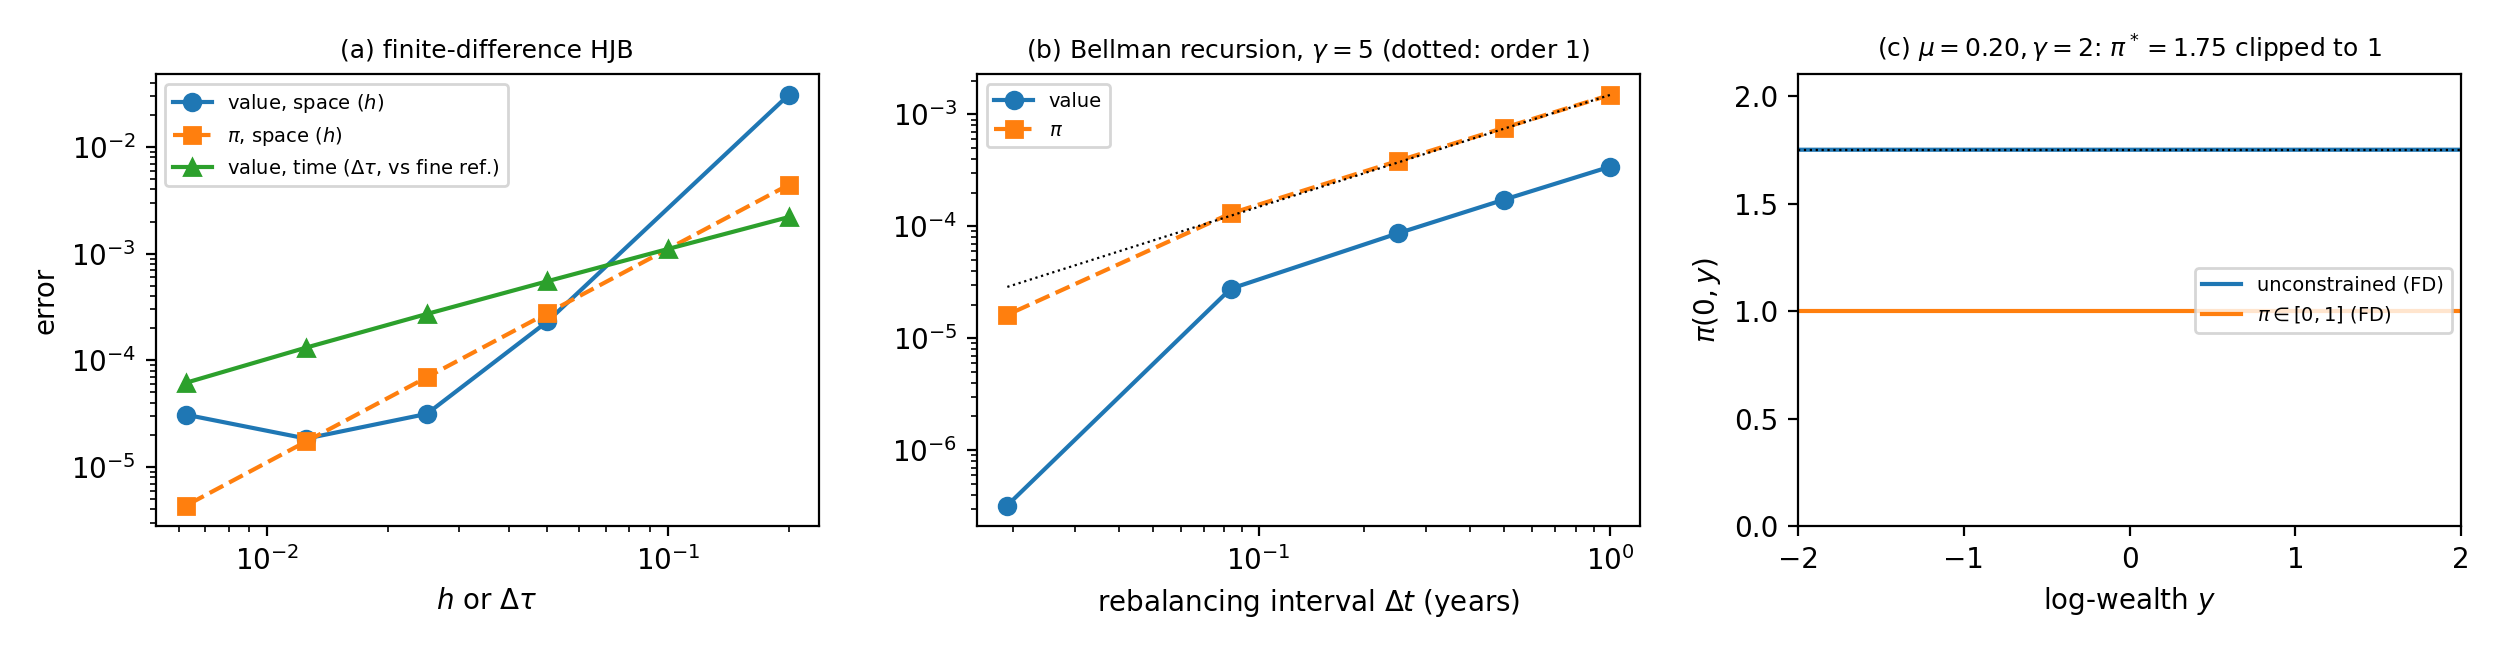
\includegraphics[width=\linewidth]{../figures/fig_hjb.png}\caption{Numerical HJB/DP (Part 5): (a) FD errors vs grid step; (b) DP errors vs rebalancing interval; (c) FD policy with and without the constraint $\pi\in[0,1]$.}\end{figure}

\begin{figure}[!htb]\centering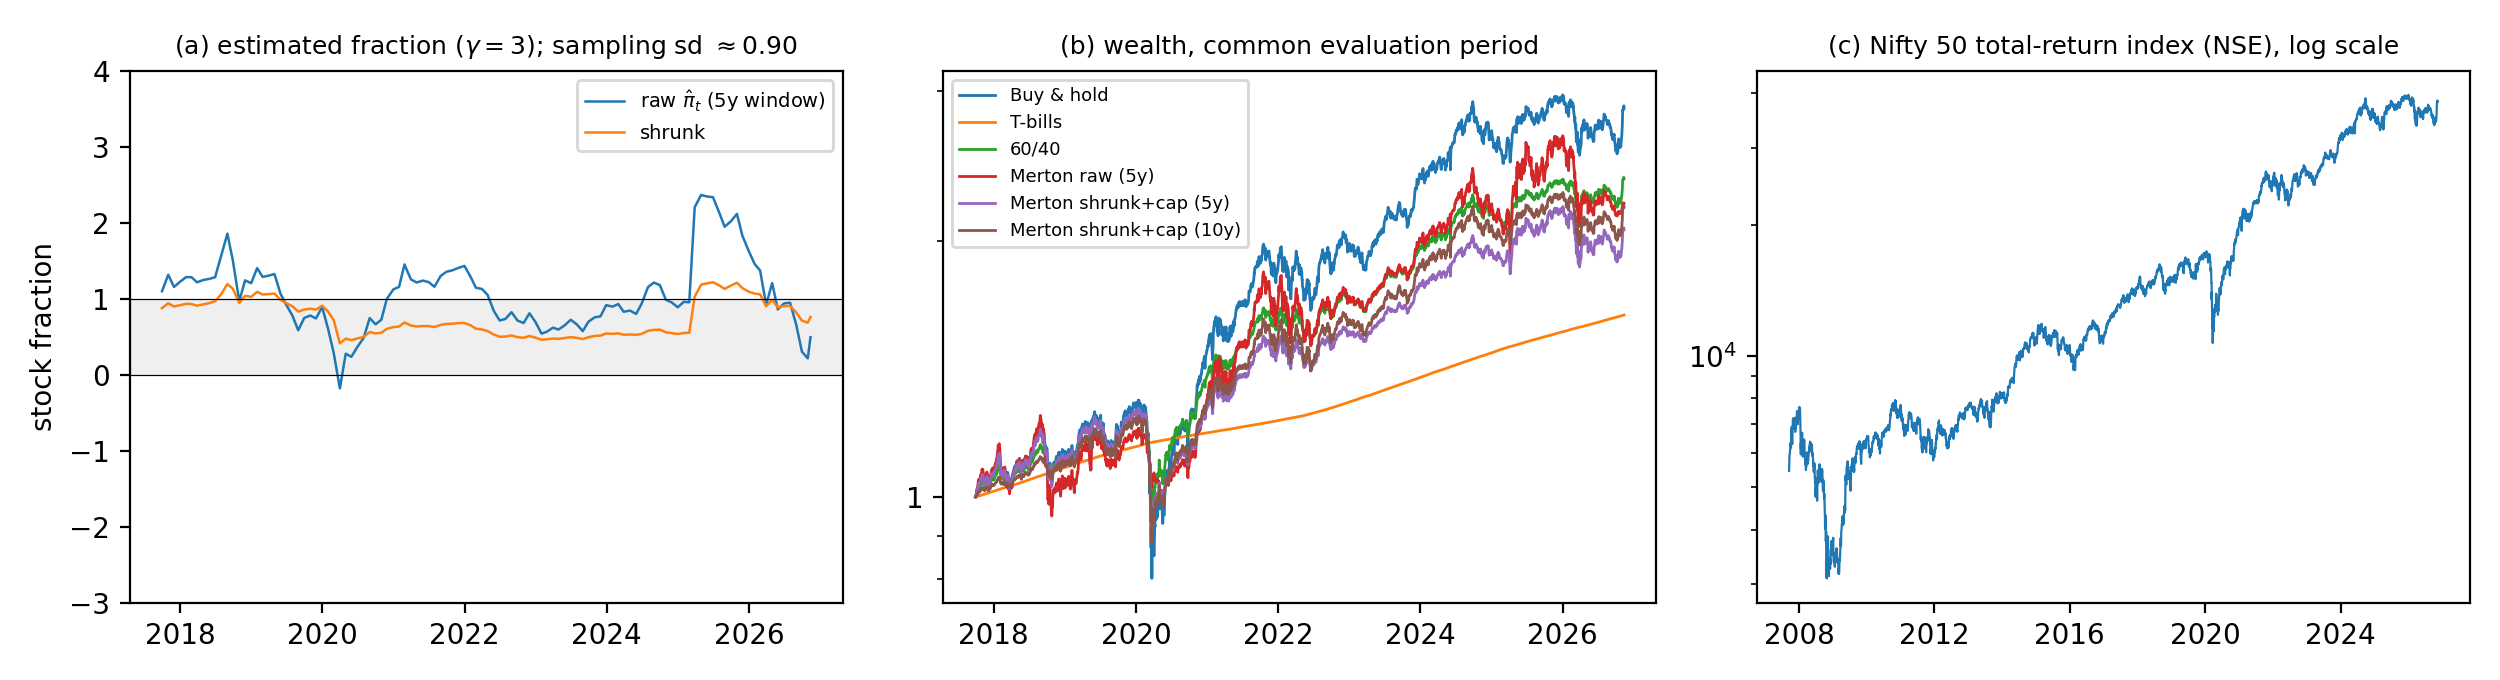
\includegraphics[width=\linewidth]{../figures/fig_data.png}\caption{Data and backtest (Part 1): (a) rolling estimated $\hat\pi$ (raw vs shrunk) with sampling band; (b) backtest wealth; (c) Nifty~50 Total Returns Index (NSE).}\end{figure}
\textbf{Real data (Nifty~50 TRI, 2007--2026).} $\hat\sigma=20.2\%$, $\hat\mu=12.2\%$, $\bar r=6.4\%$, giving $\hat\pi=0.48\pm0.38$ ($\mathrm{se}$ equal to $\sigma/(\gamma\sigma^2\sqrt{T})$): even 19.2 years cannot distinguish $\pi=0$ from $\pi=1$ at the 2$\sigma$ level. Log-returns are far from Gaussian: daily skewness $-0.29$, excess kurtosis $15.2$, Jarque--Bera $=46{,}025$ ($p\approx0$); weekly ($5.1$, JB $1096$) and monthly ($5.5$, JB $322$) returns are also rejected. $\hat\mu$ is the same at all three frequencies ($12.2/11.7/11.7\%$, se $4.4$--$4.7\%$), as $\sigma/\sqrt{T}$ predicts. Returns have mild autocorrelation (Ljung--Box $p<10^{-5}$, $\rho_1=0.03$), and squared returns are strongly dependent ($\rho_1=0.15$, $p<10^{-10}$): volatility clusters (1-year vol between 8.9\% and 47\%), which violates the constant-$\sigma$ assumption of the model. \textbf{Backtest} (Table 3; 111 rebalances, RBI T-bill $r$): the hindsight Merton fraction is $0.90$ and buys CE return $8.93\%$. No estimated rule beats the passive benchmarks: the best, 5-year capped, earns CE $8.20\%$ against $8.76\%$ for buy-and-hold and $8.70\%$ for 60/40, though with far smaller drawdown ($-15.3\%$ vs $-38.3\%$); raw rules are worst (3-year: $\pi_t\in[-0.37,2.64]$, outside $[0,1]$ on 52\% of dates, CE $-1.2\%$), and shrinking/capping helps most for short windows (3y: $-1.2\%\to4.9\%$ for shrunk+capped). The conclusion does not depend on the risk-free series: rerunning on the same period with constant $r\in\{5,6,6.5,7,8\}\%$, buy-and-hold and 60/40 beat every estimated rule at every $r$ (60/40 by up to $1.4$ points at $r=8\%$, as its cash leg earns $r$). The loss formula is an upper envelope: the dispersion of $\hat\pi$ in overlapping windows ($0.20$--$0.65$) is below the iid prediction ($0.61$--$1.21$) because windows share data and volatility mean-reverts; the 3--19 non-overlapping blocks are noisy and straddle theory ($2.1$ vs $1.6$ at 1y; $0.54$ vs $0.68$ at 5y), so $1/(\gamma\sigma\sqrt T)$ is an order of magnitude, not a forecast.
\begin{table}[!htb]\centering\footnotesize\caption{Backtest, Sep-2017--Nov-2026, monthly rebalancing, $\gamma{=}3$, RBI 91-day T-bill $r$ (mean $5.5\%$). CE = realised certainty-equivalent return. All 16 rules in \texttt{results/part1\_backtest.csv}.}
\begin{tabular}{lrrrrr}\toprule
strategy & CAGR & vol & Sharpe & max DD & CE\\\midrule
Buy \& hold Nifty 50 (TRI) & 12.2\% & 16.7\% & 0.46 & $-38.3\%$ & 8.76\%\\
60/40 (monthly) & 9.9\% & 9.8\% & 0.47 & $-23.4\%$ & 8.70\%\\
T-bills & 5.5\% & 0.1\% & -- & 0 & 5.52\%\\
Merton, 5y window, capped $[0,1]$ & 9.9\% & 12.5\% & 0.39 & $-15.3\%$ & 8.20\%\\
Merton, 10y window, shrunk & 9.0\% & 11.5\% & 0.34 & $-29.0\%$ & 7.37\%\\
Merton, 3y window, raw & 3.5\% & 19.3\% & $-0.01$ & $-45.1\%$ & $-1.15\%$\\
Hindsight Merton ($\pi=0.90$, uses future data) & 11.7\% & 14.8\% & 0.46 & $-34.5\%$ & 8.93\%\\\bottomrule\end{tabular}\end{table}

\begin{figure}[!htb]\centering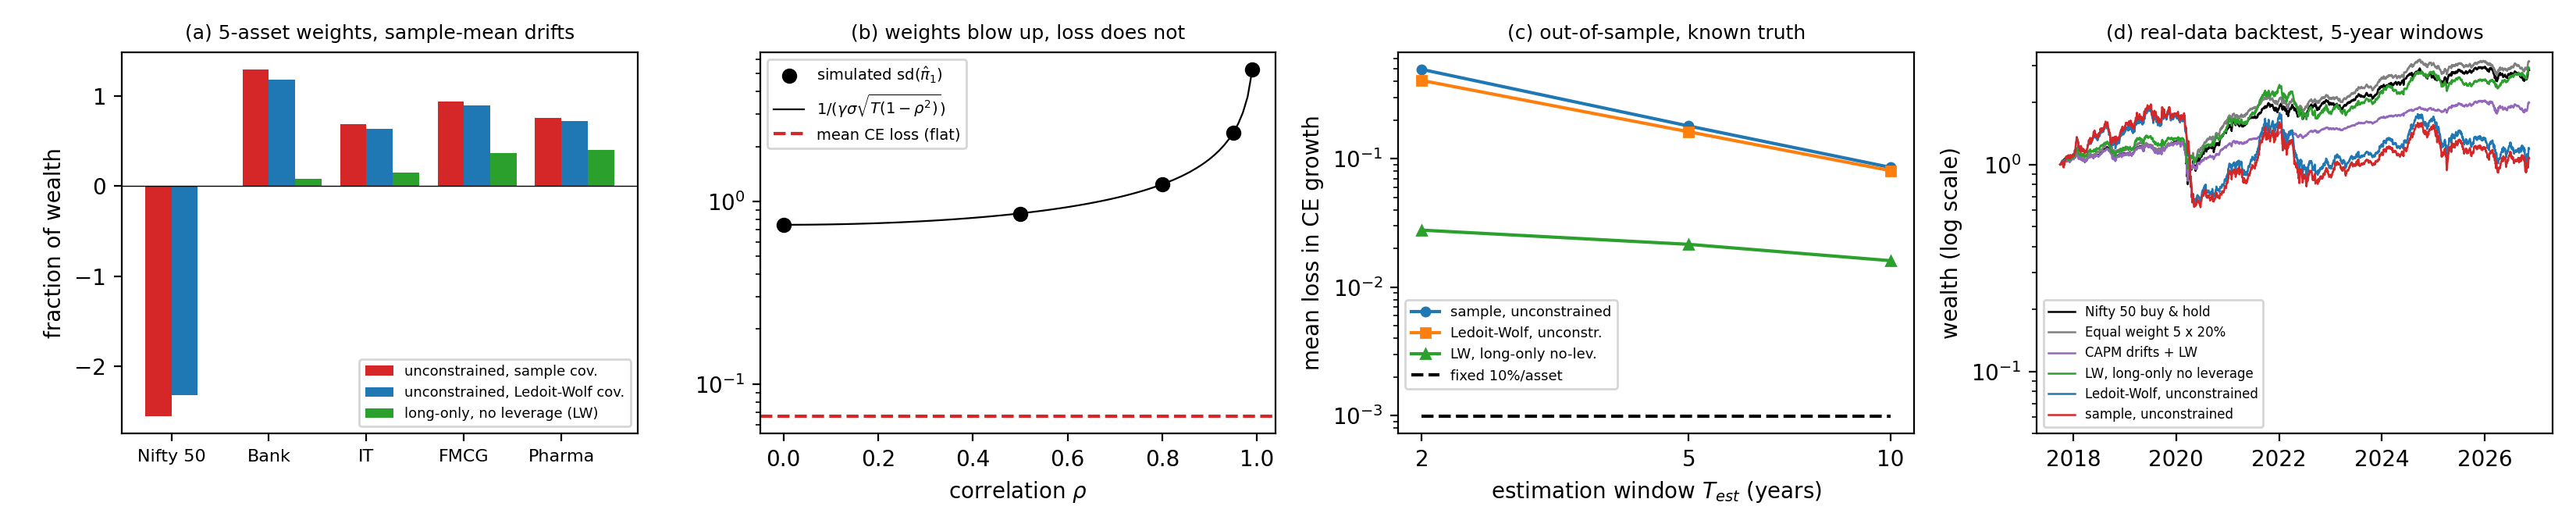
\includegraphics[width=\linewidth]{../figures/fig_multi.png}\caption{Multi-asset (Part 4): (a) full-sample weights from sample drifts; (b) $\mathrm{sd}(\hat\pi_1)$ explodes with $\rho$ while loss stays at $N/(2\gamma T)$; (c) out-of-sample loss with a known truth, $N=5$; (d) real-data rolling backtest, 5-year windows (Table 4).}\end{figure}
\begin{table}[!htb]\centering\footnotesize\caption{Multi-asset rolling backtest on NSE daily TRIs (Nifty~50, Bank, IT, FMCG, Pharma), same period, rebalancing, $r$ and $\gamma$ as Table 3; 5-year estimation windows unless stated. Gross = mean $\sum_i|\pi_i|$.}
\begin{tabular}{lrrrrr}\toprule
rule & CAGR & vol & max DD & gross & CE\\\midrule
Sample drifts + sample cov., unconstrained & 0.8\% & 31.3\% & $-68.2\%$ & 5.2 & $-13.65\%$\\
Sample drifts + Ledoit--Wolf, unconstrained & 1.9\% & 30.4\% & $-65.2\%$ & 4.2 & $-11.11\%$\\
Ledoit--Wolf, long-only, no leverage & 12.4\% & 16.9\% & $-32.0\%$ & 1.0 & 8.89\%\\
CAPM drifts + Ledoit--Wolf (10y window) & 8.9\% & 10.0\% & $-27.9\%$ & 0.6 & 7.62\%\\
Equal weights, $5\times20\%$ & 13.4\% & 14.8\% & $-32.9\%$ & 1.0 & 10.70\%\\
Nifty~50 buy \& hold & 12.2\% & 16.7\% & $-38.3\%$ & 1.0 & 8.76\%\\\bottomrule\end{tabular}\end{table}
\textbf{Multi-asset.} For $N{=}1$ the multi-asset code returns exactly the one-asset $\pi^*$ and $\kappa$ (differences $<10^{-12}$). Even with 19.2 years, each sector mean has a standard error of 4--6\% a year, and the unconstrained full-sample solution is extreme: gross leverage $6.2$ (sample cov., condition number $54$) or $5.8$ (Ledoit--Wolf, $49$), short Nifty~50 at $-2.6$ against long sectors (Bank $+1.3$, FMCG $+0.9$), because Nifty~50 and Bank are highly correlated ($\rho=0.89$) and the optimiser bets on small differences in their means. As theory says, adding imperfectly correlated assets raises in-sample $\kappa$: $7.8\%\to8.5\to10.0\to12.9\to14.9\%$ as Bank, IT, FMCG and Pharma are added (long-only no leverage: $7.8\to11.0\%$), but this is in-sample. CAPM-implied drifts put almost everything in Nifty~50 itself ($0.38$; net $0.41$, the one-asset Merton fraction with a 5\% premium), since under CAPM the market portfolio is optimal. On two synthetic assets with $\rho\in\{0,.5,.8,.95,.99\}$, $\mathrm{sd}(\hat\pi_1)$ follows $1/(\gamma\sigma\sqrt{T(1-\rho^2)})$ to $<1\%$ ($0.75\to5.27$) while $\mathrm{corr}(\hat\pi_1,\hat\pi_2)\to-1$ and mean CE loss is flat at $0.066$--$0.067$ ($N/(2\gamma T)=0.0667$): estimated weights are far off, but they err along the nearly flat direction of the objective, so wealth loss is modest. In the 5-asset out-of-sample study ($T_e=5$, truth calibrated to the data): sample unconstrained loss $0.180$, Ledoit--Wolf $0.162$ (formula $0.167$: $N$, not $\Sigma$, drives the loss), long-only no-leverage $0.022$, fixed 10\% per asset $0.001$. \textbf{The real-data backtest agrees} (Table 4): unconstrained rules run 4--5$\times$ gross leverage and lose ($-11$ to $-14\%$ CE, drawdowns near $-65\%$); long-only no leverage just beats Nifty buy-and-hold ($8.89\%$ vs $8.76\%$); and naive equal weights are best ($10.70\%$, Sharpe $0.57$), the 1/N result of \cite{dm} on Indian data. Constraints reduce the loss far more than better covariance estimation does.

\section{Conclusions}
(i) The Merton fraction $\pi^*=(\mu-r)/(\gamma\sigma^2)$ and value function (1) are reproduced by four independent routes (HJB, martingale, Monte Carlo, finite differences/DP) to the stated accuracies, and the orders of convergence agree with theory (strong: Milstein 1, EM 1/2; weak: both 1; MC $-1/2$; FD 2/1; DP 1). (ii) In practice the limiting factor is estimation error: expected loss $N/(2\gamma T_e)$ is large (0.17 CE-return-points for $N{=}5$, $T_e{=}5$) relative to any plausible gain, and in the 2017--2026 Nifty~50 backtest no estimated rule beat buy-and-hold or 60/40 at any risk-free rate; the best (5-year capped) trails by about half a point a year but halves the drawdown. With five sectors, unconstrained Merton weights lose heavily and equal weights win. (iii) Shrinkage and constraints reduce loss by factors of 3--10 at the price of a bias that is irrelevant at these sample sizes. (iv) Limitations: constant-$\sigma$ model against clear volatility clustering and fat tails, monthly rather than continuous rebalancing, a single market and no transaction costs (which would hurt high-turnover rules most); they suggest stochastic-volatility (Heston) and robust-control extensions. Not investment advice.

\textbf{Contributions.} Shrey: Part~1 data/estimation/backtest. Harshit: Part~2 Monte Carlo. Siddh: Part~3 theory and verification. Rudraksh: Part~4 multi-asset. Amay: Part~5 HJB/DP. \textbf{Cross-checks} (as planned in the proposal): Harshit's Monte Carlo and Amay's FD/DP solvers were tested against Siddh's closed forms (Fig.~1, Tables~1--2); Rudraksh's $N$-asset code against the one-asset rule ($N{=}1$ identical to $10^{-12}$); Shrey's backtest against the loss formula $1/(2\gamma T_e)$ (Section~3). Code: \texttt{src/run\_all.py} reproduces every table and figure in a few minutes.

\begin{multicols}{2}
\begin{thebibliography}{99}\footnotesize\setlength{\itemsep}{-1pt}
\bibitem{merton69} R.\ Merton, Lifetime portfolio selection under uncertainty, \emph{Rev.\ Econ.\ Stat.} 51 (1969).
\bibitem{merton71} R.\ Merton, Optimum consumption and portfolio rules in a continuous-time model, \emph{J.\ Econ.\ Theory} 3 (1971).
\bibitem{samuelson} P.\ Samuelson, Lifetime portfolio selection by dynamic stochastic programming, \emph{Rev.\ Econ.\ Stat.} 51 (1969).
\bibitem{merton80} R.\ Merton, On estimating the expected return on the market, \emph{J.\ Fin.\ Econ.} 8 (1980).
\bibitem{kls} I.\ Karatzas, J.\ Lehoczky, S.\ Shreve, Optimal portfolio and consumption decisions, \emph{SIAM J.\ Control Optim.} 25 (1987).
\bibitem{ks} I.\ Karatzas, S.\ Shreve, \emph{Methods of Mathematical Finance}, Springer 1998.
\bibitem{oks} B.\ {\O}ksendal, \emph{Stochastic Differential Equations}, 6th ed., Springer 2003.
\bibitem{pham} H.\ Pham, \emph{Continuous-time Stochastic Control and Optimization with Financial Applications}, Springer 2009.
\bibitem{kp} P.\ Kloeden, E.\ Platen, \emph{Numerical Solution of SDEs}, Springer 1992.
\bibitem{glass} P.\ Glasserman, \emph{Monte Carlo Methods in Financial Engineering}, Springer 2004.
\bibitem{dm} V.\ DeMiguel, L.\ Garlappi, R.\ Uppal, Optimal versus naive diversification, \emph{Rev.\ Fin.\ Stud.} 22 (2009).
\bibitem{lw} O.\ Ledoit, M.\ Wolf, A well-conditioned estimator for large covariance matrices, \emph{J.\ Multivar.\ Anal.} 88 (2004).
\bibitem{tapetide} TapeTide, NSE-official weekly index closes, accessed Nov 2026.
\bibitem{nifty} NSE Indices Ltd., \emph{Total Returns Index Values} (Nifty 50, Bank, IT, FMCG, Pharma), niftyindices.com, Nov 2026.
\bibitem{rbi} Reserve Bank of India, \emph{Auctions of 91-Day Treasury Bills}, 1993--2026.
\end{thebibliography}
\end{multicols}
\end{document}
